%%%%%%%%%%%%%%%%%%%%%%%%%%%%%%%%%%%%%%%%%%%%%%%%%%%%%%%%%%%%%%%%%%%%%%%%%%
%% This is a document template for an Otago thesis (Masters or PhD).
%% A skeleton chapter layout is also suggested.
%%
%% Look in the directory example_document for filled-out chapters
%% that show you how to do figures, bibliographies, and tables.
%%
%% Since this was written for Computer Science at Otago University,
%% Harvard (author, date) style citations are used.  Other students
%% should consult their advisors as to what style of citations to use.  
%%
%% This template was created by Nathan Rountree 9/2/98
%% Updates have since been made by others in the department.
%%
%%%%%%%%%%%%%%%%%%%%%%%%%%%%%%%%%%%%%%%%%%%%%%%%%%%%%%%%%%%%%%%%%%%%%%%%%%%

%%
%% In the style of a technical report, in 12pt and one sided.
%% Start chapters on right hand side pages only.
%%
\documentclass[12pt]{report}    
%%\documentclass[12pt,twoside,openright]{report} %% Use this for twosided.

%%
%% Load packages.
%%
\usepackage[bschons,nolibrary]{otagothesis}     %% Use Otago page layout
%% Use [bschons] for BScHons thesis
%%     [msc]     for MSc
%%     [phd]     for PhD 
%%     [dipsci]  for PGDipSci
%%  nolibrary-option omits a library declaration form.

\usepackage[longnamesfirst,round]{natbib} %% Use Natural Sciences bibliography

\usepackage[T1]{fontenc} %% assist clipboard copy from PDF; allow < | > etc.
\usepackage[utf8]{inputenc} %% allow UTF-8 conent in source files

%%\usepackage{times}              %% Times PostScript font. Don't use
				  %% if thesis contains lots of math.

\usepackage{graphicx}             %% jpg, gif, tiff, and pdf graphics
\usepackage{moreverb}             %% Verbatim Code Listings

% Standard Physics additions
\usepackage{amssymb,amsmath}
\usepackage{siunitx}
\usepackage[colorlinks=true,pdfstartview=FitV,linkcolor=blue, 
            citecolor=blue,urlcolor=blue]{hyperref}

%%
%% Set title, author and date.
%%
\title{Your thesis title here} % <-- Your thesis title here
\author{Your name here} % <-- Add your name here
\date{\today} % <-- Submission date here. 

%%
%% The library want to know all sorts of personal stuff!
%% Can be left out if you don't use the \frontstuff command
%%
\fullname{Your full name here} % <-- Add your name here
\department{Department of Physics}
%\dob{1 January 1900} %% date-of-birth, only needed for library declaration
\address{730 Cumberland Street, Dunedin, NZ}

%%
%% Uncomment to just print up a few chapters.
%%
%%\includeonly{literature,conclusion}

%%
%% Go!
%%
\begin{document}

%%
%% Put in titlepage and contents, etc...
%%
\frontstuff

%%
%% Set to one-and-a-half line-spacing
%%
\linespread{1.3} \normalsize

%%
%% Include each chapter as a separate file.
%% These lines assume there are files called intro.tex, literature.tex etc.
%%
\chapter{Introduction}
\label{chap:intro}

This is the first chapter.  Here is an example citation:
\citet{rountree98}.


\chapter{Literature Survey}
\label{chap:bib}

Since this chapter would normally contain your literature review and
background sections, it seems like a good time to discuss citations
and bibliographies.  The file {\tt thesis.tex} is set to use Harvard
style citations, using the \verb|natbib| package.
The following sections describe how to use this package effectively.

\section{Reference Lists}

The {\tt otagothesis} package automatically renames your selected
bibliography to ``References'', since in Computer Science we only list
works that are actually referred to in the text.  We use the Harvard
style of citations as implemented by the \verb|natbib| package, which
is part of the TeTeX distribution of LaTeX (i.e.\ the one found on
most versions of Linux).

To get all references and citations correct, you need to perform the
\LaTeX\ stanza (see Subsection~\ref{subsec:trouble}): {\tt pdflatex,
bibtex, pdflatex, pdflatex}.  The makefile does this for you when you type
{\tt make}.

Every time you use a \verb|\citet| or \verb|\citep| command, a
bibliographic entry
will be added to your reference list.  On the whole, BibTeX will get
the styles correct, but you should definitely check this before
submitting a final copy; BibTeX bibliographies are notoriously
difficult to spell-check and some strange things can happen with
capitalisation.

\section{Creating a Bibliography File}

If you look at the file {\tt thesis.bib} you will find some
instructions on how to create a BibTeX database, and some sample
entries.  The makefile and thesis template are set up so as to
{\em expect} to see a file called {\tt thesis.bib} (your bibliographic
database file) and will generate an error message if there isn't one.
You can find a large number of Computer Science citations in
BibTeX format on the Collection of Computer Science Bibliographies
Homepage, at {\tt http://liinwww.ira.uka.de/bibliography/}.

A bibliographic entry looks something like this:

\linespread{1} \small
\begin{quote}
\begin{verbatim}
@InProceedings{amir97,
  author = 	 {Amihood Amir and Ronen Feldman and Reuven Kashi},
  title = 	 {{A New and Versatile Method for Association Generation}},
  booktitle = 	 {{Principles of Data Mining and Knowledge Engineering;
                   First European Symposium, PKDD'97}},
  OPTcrossref =  {},
  OPTkey = 	 {},
  editor = 	 {Jan Komorowsk and Jan Zytkow},
  OPTvolume = 	 {},
  OPTnumber = 	 {},
  OPTseries = 	 {},
  year = 	 {1997},
  OPTorganization = {},
  publisher = {Springer-Verlag},
  address = 	 {Trondheim, Norway},
  month = 	 {June},
  pages = 	 {221--231},
  OPTnote = 	 {},
  OPTannote = 	 {}
}
\end{verbatim}
\end{quote}

\linespread{1.3} \normalsize
Separate authors with the word ``and''.  The title is in double
braces to maintain the capitalisation exactly as written, as is the
title of the conference proceedings.  The very first part of the entry
(amir97) must be a unique key---this is what you will use when
referencing the work in your document, so make it something easy to
remember.  Most people use something like ``first\_author\_year'' with
a letter tacked on the end to avoid duplicates (e.g. amir97a, amir97b).

Here are some suggestions for creating your own database:
\begin{itemize}
\item Leave optional fields in place, even when they are empty.  You
never know when that information might turn up, so all you have to do
is add it into the correct field and remove the OPT prefix.
\item Use double braces to maintain your own capitalisation.
You can always remove them later using a search-and-replace, but it is
a real pain to go through the database putting them in.
\item Use the emacs macro to create each new entry (M-x bib-TAB-TAB
for a list of options).  You will be thankful for the consistency as
the list grows.
\item Use ``@InProceedings'' for an article in conference proceedings, not
``@Proceedings''.  Use ``@InCollection'' for an article which forms a
stand-alone chapter in a book where each chapter is written by a
different author, not ``@InBook''.
\end{itemize}


\section{Citation Styles}

The most usual form of citation is an ``aside'' (in parentheses, like
this). The time to use it is when you have made a statement which
might be questionable, and you wish to give a source for it. For
instance:
\begin{quote}
Writing a thesis is easy \citep{rountree98}.
\end{quote}
This type of citation is made using the \verb|\citep| command.  It
should be used sparingly, because it lends itself most to sweeping,
general statements (of which you don't want too many!).

The {\tt natbib} package gives you another option with
the \verb|\citet| command.  This enables you to refer directly
to a piece of work, using it as a noun in your sentence.  For
instance:
\begin{quote}
The article by \citet{amir97} describes a method of preprocessing
a database into a trie, so as to make association generation much quicker.
\end{quote}
This style is more versatile, and should be favoured over the use of
\verb|\citep|.

When there are multiple authors, all subsequent citations of that work
will just list the first author followed by ``et al.''.  This will happen\
automatically; for instance:
\begin{quote}
Here is a second citation of \citet{amir97}.
\end{quote}
If for some reason you want the whole list of authors, you can use the
``starred'' form of the command, i.e. \verb|\citep*| or
\verb|\citet*|. 

Sometimes, it will be inelegant to include the year with the
citation; for example when you are referring to a particular article
very frequently in a single section, (perhaps when a chapter forms a
criticism of another piece of work).  For those purposes, use the command
\verb|\citeauthor|.  This will allow a sentence like ``the
book is of no use to anyone, but \citeauthor{rountree98} published it
anyway.''

The command \verb|\citeyear| is similar, but gives just the year,
allowing you to occasionally break style if you wish---and
\verb|\citeyearpar| will give the year with parentheses.  This will
let you write a sentence like ``\citeauthor{amir97}'s article, published
in \citeyear{amir97}, is the most up-to-date treatment of this topic.''

If you wish to add text to the citation (for instance the letters
e.g., or some page numbers), you may do so either at the beginning or
the end.  For the end (as with page numbers), simply add an optional
argument; \verb|\citep[pp97--100]{rountree98}| will produce
\begin{quote}
The section titled ``Are You Bored Yet?'' is particularly useless
\citep[pp97--100]{rountree98}.
\end{quote}
However if you want to add text at the beginning of the citation, you
should use a combination of the \verb|\citetext| and \verb|\citealp|
commands, like this:
\begin{verbatim}
Several works have been cited in this document
\citetext{e.g., \citealp{rountree98,amir97}}.
\end{verbatim}
producing:
\begin{quote}
Several works have been cited in this document
\citetext{e.g., \citealp{rountree98,amir97}}.
\end{quote}

Citing your current thesis is not allowed.  It is acceptable to refer to
previous work of your own. 


\chapter{A New Approach}
\label{chap:new}


\chapter{Implementation}
\label{chap:implementation}


\chapter{Results}
\label{chap:tables}

Chapters containing experimental results often contain a number of
tables.  These are ``floated'' in \LaTeX, just like figures.  The
short caption is automatically added to the ``List of Tables'' page,
and---like a figure---the table can contain almost anything
(graphics, text, tabular material, code snippets or whatever).

The most important thing to establish is the difference between
the {\tt table} and {\tt tabular} environments.  A table is just a
floating body, but the tabular environment is used to create
{\em actual} tables.  The following examples show what you can do with
both environments.

\section{The {\tt table} Environment}

Table~\ref{tab:ex1} is an example of a table with graphical content.
Note one convention:  unlike figures, tables are usually captioned at
the {\bf top}, not the bottom.  

As with figures, the best place to put the \verb|\label| is directly
after the \verb|\caption|, otherwise you will end up with the section
label instead.  You can find the code for Table ~\ref{tab:ex1} on page~42,
starting at line~106.

\section{The {\tt tabular} Environment}

Most likely what you will want to put inside a {\tt table} environment
is a table of data.  This is done using the {\tt tabular} environment,
as in the following example.  This code:

\linespread{1}\small
\begin{quote}
\begin{verbatim}
\begin{tabular}{l|c|c}
Day & Cups of Coffee & Lines of Code \\
\hline
Mon & 3 & 200 \\
Tue & 5 & 500 \\
Wed & 5 & 300 \\
Thu & 4 & 200 \\
Fri & 3 & 100 \\
\end{tabular}
\end{verbatim}
\end{quote}
\linespread{1.3}\normalsize

will produce this table:

\begin{center}
\begin{tabular}{l|c|c}
Day & Cups of Coffee & Lines of Code \\
\hline
Mon & 3 & 200 \\
Tue & 5 & 500 \\
Wed & 5 & 300 \\
Thu & 4 & 200 \\
Fri & 3 & 100 \\
\end{tabular}
\end{center}

The vertical bars in the \verb+{l|c|c}+ argument tell \LaTeX\ to put
lines between each column. The argument \verb+{|l|c|c|}+ would have
resulted in lines around the outside as well. The letters indicate the
text formatting in the table (l for left, c for center, etc.).  The
command \verb|\hline| is used to add horizontal lines (including at
the top and bottom of the table) and \verb|\\| is used to end each
row.  You do not need to use \verb|\\| at the end of \verb|\hline|.
Finally, the {\tt \&} character is used to separate entries within
rows.

Table~\ref{tab:ex2} is a slightly more complex example of tabular
material, included as a table in the document.  Here is the code which
produced it:

\linespread{1}\small
\begin{quote}
\begin{listing}{1}
\begin{table}
\hrulefill
\caption[A tabular table]{An example of a table whose contents are
formatted using the {\tt tabular} environment.}
\label{tab:ex2}
\hrulefill
\begin{center}
\begin{tabular}{|l|l|r|} \hline\hline
{\em type} & \multicolumn{2}{c|}{\em style} \\ \hline
smart & red & short \\
rather silly & puce & tall \\ \hline\hline
\end{tabular}
\end{center}
\par
\bigskip
\hrulefill
\end{table}
\end{listing}
\end{quote}
\linespread{1.3}\normalsize

The \verb|\multicolumn| command on line 8 allows the spread of data
over several columns, and overrides the normal vertical bar placement.
Lines 2, 6 and 14--16 produce the horizontal lines which separate
the table from the rest of the text.

\begin{table}
\hrulefill
\caption[A table with graphical input]{An example of a table which
uses graphical input as its content.  This is once again the
contents page of this document, saved as PDF.}
\label{tab:ex1}
\hrulefill
\begin{center}
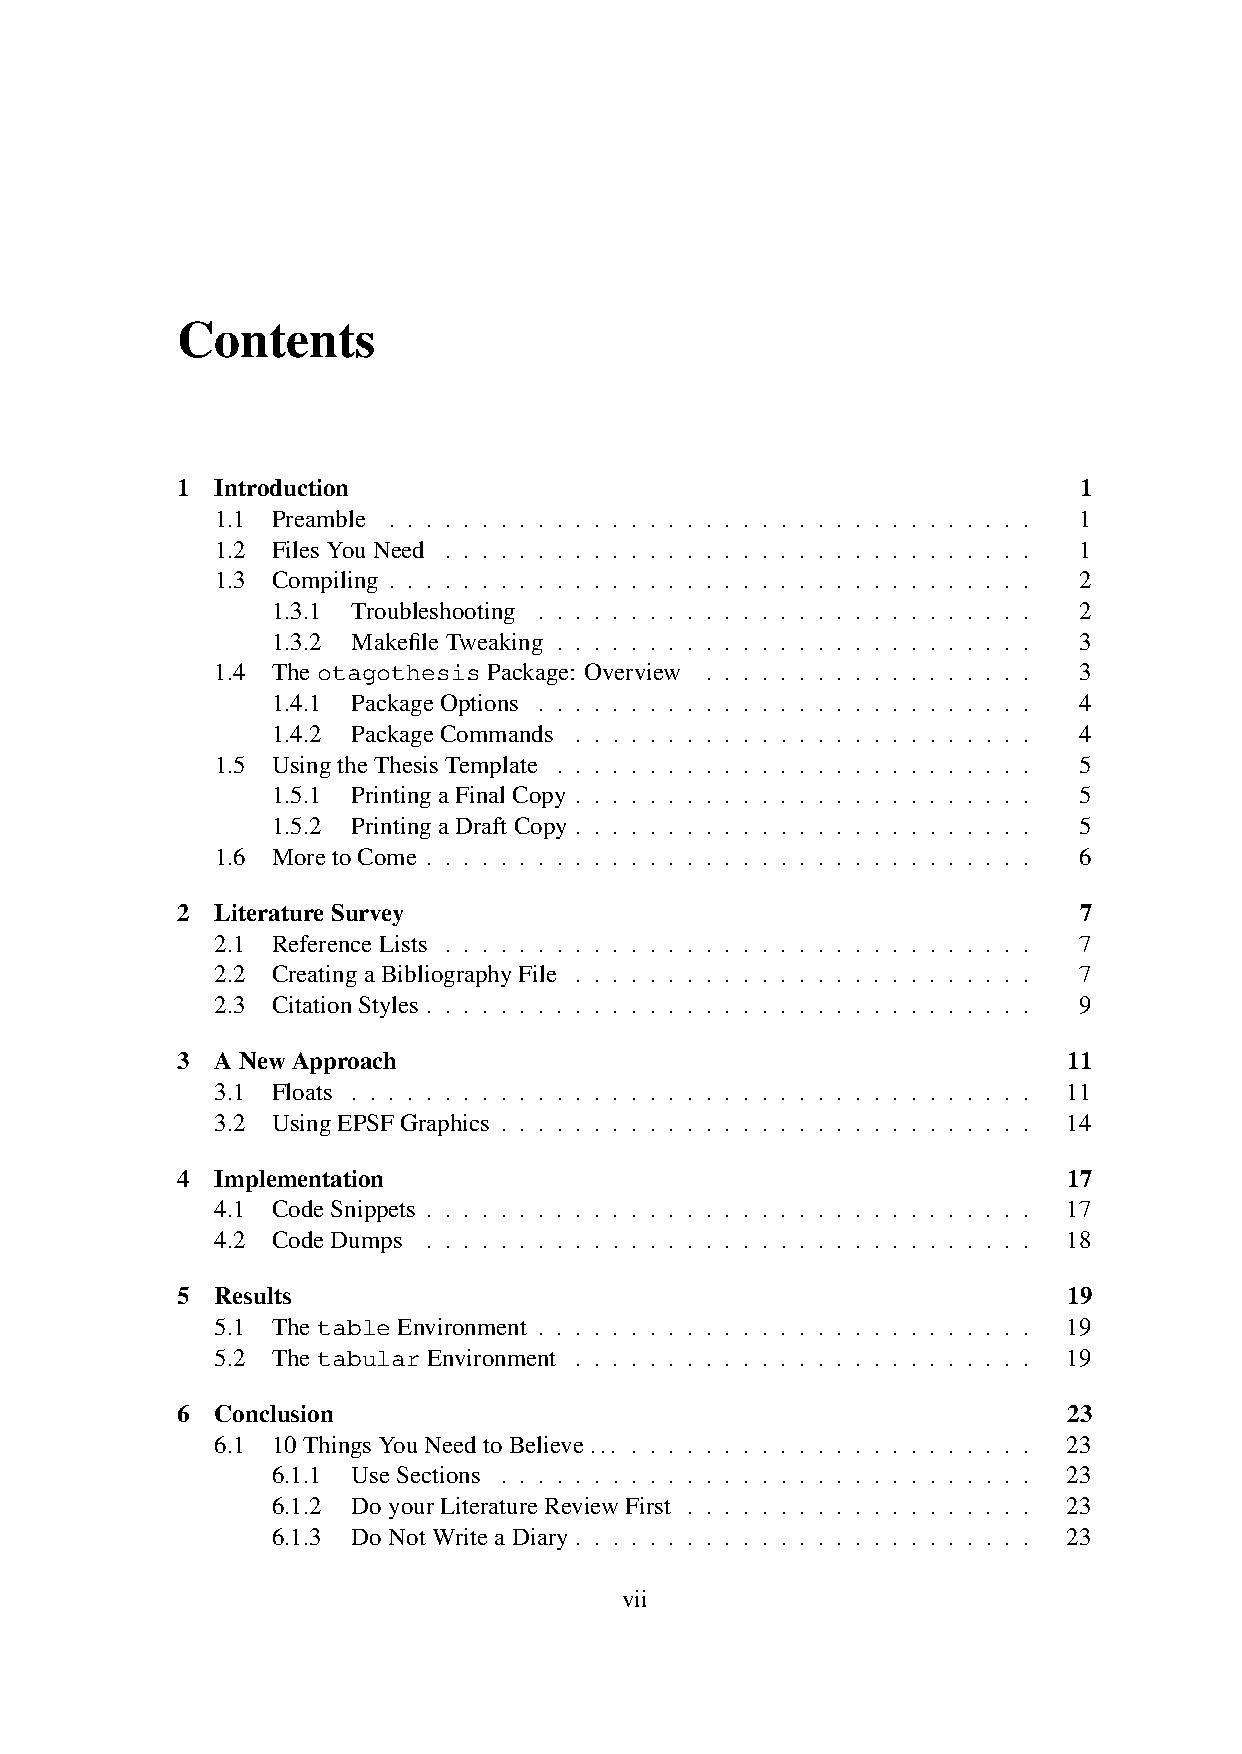
\includegraphics[scale = 0.5, angle = 270]{page.pdf}
\end{center}
\par
\bigskip
\hrulefill
\end{table}


\begin{table}
\hrulefill
\caption[A tabular table]{An example of a table whose contents are
formatted using the {\tt tabular} environment.}
\label{tab:ex2}
\hrulefill
\begin{center}
\begin{tabular}{|l|l|r|}
\hline\hline
{\em type} & \multicolumn{2}{c|}{\em style} \\ \hline
smart & red & short \\
rather silly & puce & tall \\ \hline\hline
\end{tabular}
\par
\bigskip
\hrulefill
\end{center}
\end{table}


\chapter{Conclusion}
\label{chap:final}

Here are some final comments about putting together a thesis.  They
are mostly opinion (and certainly opinionated) so take on board what
you will.  This is free advice after all (and may be worth as much)
but it is meant to make life easier for you.

\section{10 Things You Need to Believe \ldots}
\subsection{Use Sections}
Chapters are BIG things.  Write an opening paragraph to your chapter,
then mark in each section you are going to cover.  Fill in the actual
content AFTER you have worked out just what the sections are going to
be.

\subsection{Do your Literature Review First}
Lots of people do their literature review after they have written
their program/done their experiment.  Don't fall into this trap---you
think the write-up will only take six weeks, but it won't, because
the lit.\ review will take four.  Create a BibTeX file while you do
the review, so you can cite as you go.  You would be amazed at how
many people don't do this.

\subsection{Do Not Write a Diary}
Nobody is interested in how you went about writing your program.  The
academic community is interested in how you have integrated the
existing theory with your own ideas, and the department is interested
in why you made particular design decisions.  Remember that we are a
Humanities department as well as a Science department, so we want to
see some sort of convincing argument for your ideas.

\subsection{Avoid Visual Formatting}
Try not to use commands like \verb|\vspace, \pagebreak| or
\verb|\enlargethispage|.  The whole point of \LaTeX\ is that it
provides a markup language that works perfectly 90\% of the time.
This means that when you have {\bf finished}, the last thing you
should do is print up a draft, then go through and mark any formatting
you don't like (there will probably be about one thing every ten
pages).  That is the time to insert things like \verb|\pagebreak|
commands.

\subsection{Learn \LaTeX\ Early}
The learning curve for \LaTeX\ is steep but short.  The idea is that
some poor sod like me does all the dirty work, and all you have to do
is {\em fill in the content}.  However you may spend about a week
learning all the fiddly bits (like tables and figures), and you don't
want to be taking time away from the actual thesis writing.

\subsection{Read Some Documentation}
In the Systems Lab, we are going to make every attempt to have
printed documentation lying around.  If you need quick help, check out
the file {\tt essential.dvi} on any Linux \LaTeX\ installation.  It
is probably the best short guide to \LaTeX\ around, and even contains
lots of tricky maths examples.

\subsection{Save Paper}
On a mac, use the layout options to print two-up and double-sided. On a
linux machine, use {\tt  psutils} to print your drafts.  This way you
use a quarter of the paper.  Here's what to do if you don't have
a duplex printer:
\begin{enumerate}
\item Use the twosided option and make the PDF file.
\item Use \verb|pdftops| to convert \verb|thesis.pdf| to \verb|thesis.ps|.
\item Use {\tt psbook} to arrange the pages for booklet printing;
\begin{quote}
e.g. {\tt psbook thesis.ps thesis.bk.ps}.
\end{quote}
\item Use {\tt psnup} to get the book to a booklet;
\begin{quote}
e.g. {\tt psnup -2 thesis.bk.ps thesis.2up.bk.ps}.
\end{quote}
\item Use {\tt psselect} to print up the even pages first (in reverse),
then the odd pages;
\begin{quote}
e.g.\\
type {\tt psselect -e -r thesis.2up.bk.ps | lpr}\\
Put the result into the sheet feeder, blank side up\\
type {\tt psselect -o thesis.2up.bk.ps | lpr}\\
\end{quote}
\end{enumerate}

That's the theory; in practice it goes something like this:
\begin{quote}
{\tt psbook thesis.ps | psnup -2 | psselect -e -r | lpr}\\
Now open the laserjet side-door and put the paper which came out after
the first command on the tray.  Don't change its orientation or
anything: just pick it up, move it to the tray and drop it.  Then:\\
{\tt psbook thesis.ps | psnup -2 | psselect -o | lpr}\\
\end{quote}

\subsection{Use \LaTeX, not Word}
Microsoft Word is not your friend.  Word is not {\em anybody's} friend.
It is possible to write large documents in Word, but you have to be
{\bf so} strict on yourself (using heading styles, TOC entries, etc.)
that you may as well have used \LaTeX\ in the end anyway.  Once a
problem is nailed in \LaTeX, it stays nailed.  The same is not true of
Word.  Pdflatex produces standard PDF which can be
printed anywhere, and is fast becoming a standard for on-line article
publication.  Ask anyone how many problems they have had printing Word
documents to PostScript printers.

\subsection{The First Copy is Not the Final Copy}
Well, unless you're Isaac Asimov, or Mozart. Print up
draft copies of chapters and give them to your supervisor to read,
then implement any changes when they get returned.  Then, a week
later, reread the chapter and change anything that makes you cringe.

\subsection{Spell Check your Work}
If you are using UNIX (as I have assumed throughout this document)
then the {\tt ispell} program is a pretty good spell checker.  Also
get someone to check your punctuation and grammar, and be on the
lookout for spellchecker errors (like ``fro'' instead of ``for'',
which will not be picked up at all).  Even the {\em worst} writer of
novels who gets published has a good grasp of grammar, because it is
unpleasant to read work which doesn't make sense.  There is no point
in putting the examiner in a bad mood by turning the reading of your
thesis into an unpleasant chore.

\section{General Comments}
Traditionally, academic works are written using the passive
voice---``this was done'' rather than ``we did this''.  Also, the use
of the personal pronoun ``I'' is avoided in favour of ``we''; but here
you must be careful.  There are two ways of using ``we'': either {\em
in}clusively or {\em ex}clusively.  Inclusively is pretty much alright
as it makes the reader feel like part of the story; e.g. ``Reducing
Equation 2.3 to Equation 2.4, we can see \ldots''.  Exclusively sounds
pompous---``we now present a new algorithm which will solve this
problem \ldots'' and should be avoided unless writing a paper with
more than one author.

There are some other things worth remembering:
\begin{itemize}
\item When referring to another chapter or section, Use a capital
letter; e.g. ``see Chapter~3'' not ``see chapter~3''.  Use a tilde
character $(\sim)$ to put a non-breaking space before the number.  That
way you will never begin a new line with the number.
\item The layout suggested in this document (introduction, lit.\
review, new ideas, implementation, results, conclusion) is pretty
generic.  If you stick to it, you will complete a thorough but boring
thesis.  You will almost certainly need to digress occasionally, and
perhaps integrate the literature review more with your own work.
While academic writing isn't usually noted for its racey prose, it
doesn't have to be boring.
\end{itemize}

Finally, at the end of your thesis, don't be afraid to blow your own
trumpet.  If you have done something new and original, restate just
what that is.  The last part of the concluding chapter is what most
people read straight after the abstract, so it has to be just as pithy
and imagination-capturing.


%%
%% Make certain the ``references'' section begins on a recto page when
%% document is double-sided.
%% The ``bibliography'' line assumes that there is a file called
%% ``thesis.bib'' and that somewhere in the chapter material you have
%% cited something from it.
%%
\cleardoublepage
\bibliographystyle{otago}
\bibliography{thesis}

%%
%% Now we have to get the source code in as a set of Appendices.
%% Source code will be Appendix A, with each file numbered X.y
%%
\appendix

%%
%% -> \chapter will cause the next bit to be labelled Appendix A
%% -> \section will give us A.1, \subsection A.1.1 etc.
%%
%% I suggest a section for each program and a subsection for each file
%% in the program.  Alternatively, a chapter for each program, a
%% section for each library and a subsection for each file.
%%
\chapter{Source Code for thesis.dvi}

You do not need to include the source code for your thesis (this is just an example).
However, including code you have written to solve numerical problems 
can be useful -- talk to your supervisor.

\linespread{1}
\footnotesize

\section{thesis.tex}
\listinginput[10]{1}{thesis.tex}

\subsection{abstract.tex}
\listinginput[10]{1}{abstract.tex}

\subsection{acknowledgements.tex}
\listinginput[10]{1}{acknowledgements.tex}

\subsection{intro.tex}
\listinginput[10]{1}{intro.tex}

\subsection{literature.tex}
\listinginput[10]{1}{literature.tex}

\subsection{new\_ideas.tex}
\listinginput[10]{1}{new_ideas.tex}

\subsection{implementation.tex}
\listinginput[10]{1}{implementation.tex}

\subsection{results.tex}
\listinginput[10]{1}{results.tex}

\subsection{conclusion.tex}
\listinginput[10]{1}{conclusion.tex}

\subsection{appendices.tex}
\listinginput[10]{1}{appendices.tex}

%%
%% \listinginput[x]{y}{filename} gives a listing of <filename>,
%% starting at line y with a line-number at every xth line.
%%


\end{document}
%% All Done!
